\documentclass[master=cws,masteroption=se,english,oneside]{kulemt}
\setup{
	title={Comparative study of tools for cross-platform mobile application development},
  	author={Michiel Staessen},
  	assessor={},
  	promotor={prof.\,dr.\,ir.\ Erik~Duval},
  	assistant={ir.\ Gonzalo~Parra}
}

% The following \setup may be removed entirely if no filing card is wanted
\setup{
	filingcard,
	translatedtitle="",
	udc=,
	shortabstract={
		Here comes a very short abstract, containing no more than 500
    		words. \LaTeX\ commands can be used here.     	}
}

% Uncomment the next line for generating the cover page
%\setup{coverpageonly}
% Uncomment the next \setup to generate only the first pages (e.g., if you
% are a Word user.
%\setup{frontpagesonly}

% Choose the main text font (e.g., Latin Modern)
\setup{
	font=utopia
}

%% Additional formatting settings
%  Use the chapter and headings styles as well as the ToC formatting
%  as defined in the kulemtx document style
\usepackage{kulemtx}
\headstyles{kulemtman}
\kulemtmanToC

% If you want to include other LaTeX packages, do it here.
\usepackage{url}

% Finally the hyperref package is used for pdf files.
% This can be commented out for printed versions.
\usepackage[pdfusetitle,colorlinks,plainpages=false]{hyperref}

\usepackage[square,numbers]{natbib}
\usepackage{amsmath}
\usepackage{amsfonts}

% Paragraph definition
\setlength{\parindent}{0pt}
\setlength{\headheight}{1.8em}
\newcommand{\npar}{\par \vspace{2.3ex plus 0.3ex minus 0.3ex}}

%\includeonly{chap-n}
\begin{document}

\begin{preface}
    % dankwoord
\end{preface}

\tableofcontents*

\begin{abstract}
    The \texttt{abstract} environment contains a more extensive overview of
    the work. But it should be limited to one page.
\end{abstract}

% A list of figures and tables is optional
%\listoffigures
%\listoftables

% If you only have a few figures and tables you can use the following instead
%\listoffiguresandtables

% The list of symbols is also optional.
% This list must be created manually, e.g., as follows:
%\chapter{List of Abbreviations and Symbols}
%\section*{Abbreviations}
%\begin{flushleft}
%  \renewcommand{\arraystretch}{1.1}
%  \begin{tabularx}{\textwidth}{@{}p{12mm}X@{}}
%    LoG   & Laplacian-of-Gaussian \\
%    MSE   & Mean Square error \\
%    PSNR  & Peak Signal-to-Noise ratio \\
%  \end{tabularx}
%\end{flushleft}
%\section*{Symbols}
%\begin{flushleft}
%  \renewcommand{\arraystretch}{1.1}
%  \begin{tabularx}{\textwidth}{@{}p{12mm}X@{}}
%    42    & ``The Answer to the Ultimate Question of Life, the Universe,
%            and Everything'' according to \cite{h2g2} \\
%    $c$   & Speed of light \\
%    $E$   & Energy \\
%    $m$   & Mass \\
%    $\pi$ & The number pi \\
%  \end{tabularx}
%\end{flushleft}

% Now comes the main text
\mainmatter

\chapter{Introduction}
\label{cha:intro}

The mobile industry is without a doubt one of the most vibrant industries at the moment. It is characterized by rapid growth and intense competition which has led to fragmentation. This chapter first presents an overview of the evolution in the mobile device landscape, then explains the problem of fragmentation and how cross-platform tools (CPTs) can help solve this problem and finally, the goals of this thesis are defined.

\section{The mobile device landscape}

Mobile phones have been around since the nineties but ever since the (nearly simultaneous) introduction of the iPhone 3G and the HTC Dream in 2008, smartphones are taking over from traditional cell phones or feature phones. A feature phone (sometimes also called a dumb phone) is a low-end mobile phone, providing only basic telephony and texting capabilities. Smartphones on the other hand are high-end devices that combine the functionality of mobile phones with the functionality of a portable computer. These devices have advanced computing power and often include multiple connectivity options (cellular, Wi-Fi, Bluetooth, NFC, etc.), sensors (GPS, compass, accelerometer, etc.), applications, etc. In the last five years, smartphone sales have grown tremendously. According to quarterly studies by Gartner\footnote{Gartner is an American research and advisory firm, specialized in information technology, \url{http://www.gartner.com}.} \citeGartner, smartphone sales have grown 544\% since the second quarter of 2008 (see \fref{fig:smartphone-sales}). Smartphones are becoming ubiquitous and in some regions like the United States, smartphone penetration\footnote{this is the ratio between smartphones and all mobile phones} has already reached more than 50\% \cite{Nielsen:2012}. 

\begin{figure}[h]
    \centering
    \includegraphics[width=\textwidth]{../resources/figs/smartphone_sales.pdf}
    	\caption{Evolution of worldwide smartphone sales by operating system (lines) and smartphone penetration (bars). Source: Gartner \citeGartner}
    	\label{fig:smartphone-sales}
\end{figure}

Each of these smartphones comes with a mobile operating system which allows owners to run third-party software, typically called applications or apps for short, on their device. These application play an important role as they drive the network effects associated with a certain platform. Applications create additional value for a platform, which attracts new users. Whenever a platform attracts more users, it becomes even more valuable. This vicious circle is called a network effect. Network effects make it hard for new platforms to gain traction which is visible in \fref{fig:smartphone-sales} and \fref{fig:smartphone-share}. Android and iOS are currently dominant (and continue growing) while other platforms are either in decline (like Symbian and Blackberry, formerly RIM) or have a hard time getting traction (like Windows Phone, the successor of Windows Mobile, which already existed before Android and iOS).

\begin{figure}[h]
    \centering
    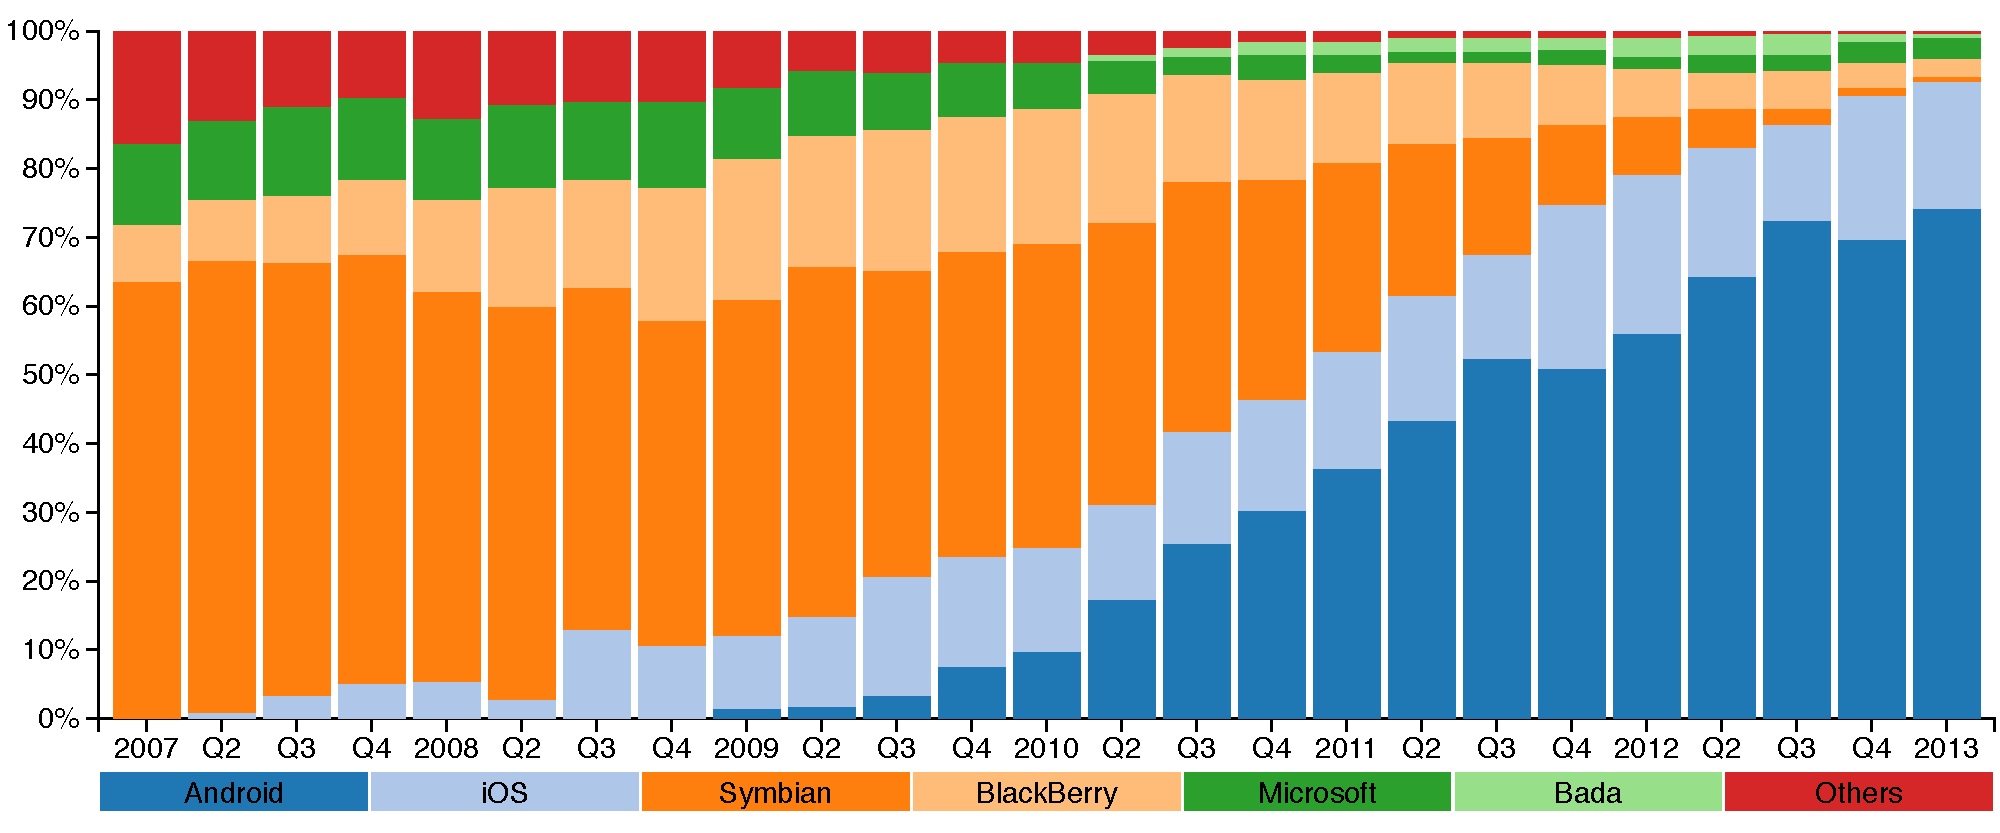
\includegraphics[width=\textwidth]{../resources/figs/smartphone_share.pdf}
    \caption{Evolution of worldwide smartphone market share by operating system.\newline Source: Gartner \citeGartner}
    \label{fig:smartphone-share}
\end{figure}

However, there is no single major platform. In addition, the IDC\footnote{International Data Corporation is another American research, analysis and advisory firm, specializing in information technology, telecommunications and consumer technology, \url{http://www.idc.com}.} predicts that Windows Phone will gain a significant market share by 2016 and that 90\% of the worldwide smartphone market will then be covered by Android, iOS and Windows Phone \cite{IDC:phone}. Hence, it is reasonable to assume that there will always be more than one major platform.

The second type of mobile devices are tablet computers or tablets. In their current form, tablets are somewhat similar to smartphones but they have larger touchscreens (customarily starting at 7 inches in diagonal) and do not offer basic telephony. However, some of them do have a cellular radio that can be used for data transmission. Because of their hardware similarities, their software is also similar: the dominant smartphone operating systems are also used in tablets.

As with smartphones, tablets gained a lot of popularity since the launch of the iPad and Android tablets. According to other studies by both Gartner \citep{Gartner:11tab,Gartner:12tab} and the IDC \citep{IDC:tablet}, tablets will continue to gain popularity and sales will be mainly driven by iPads and Android tablets (see \fref{fig:tablet}). Even though these studies disagree on which operating system will be used in most devices, they both predict there will be three major platforms: iOS, Android and Windows. 

\begin{figure}[h]
    \centering
    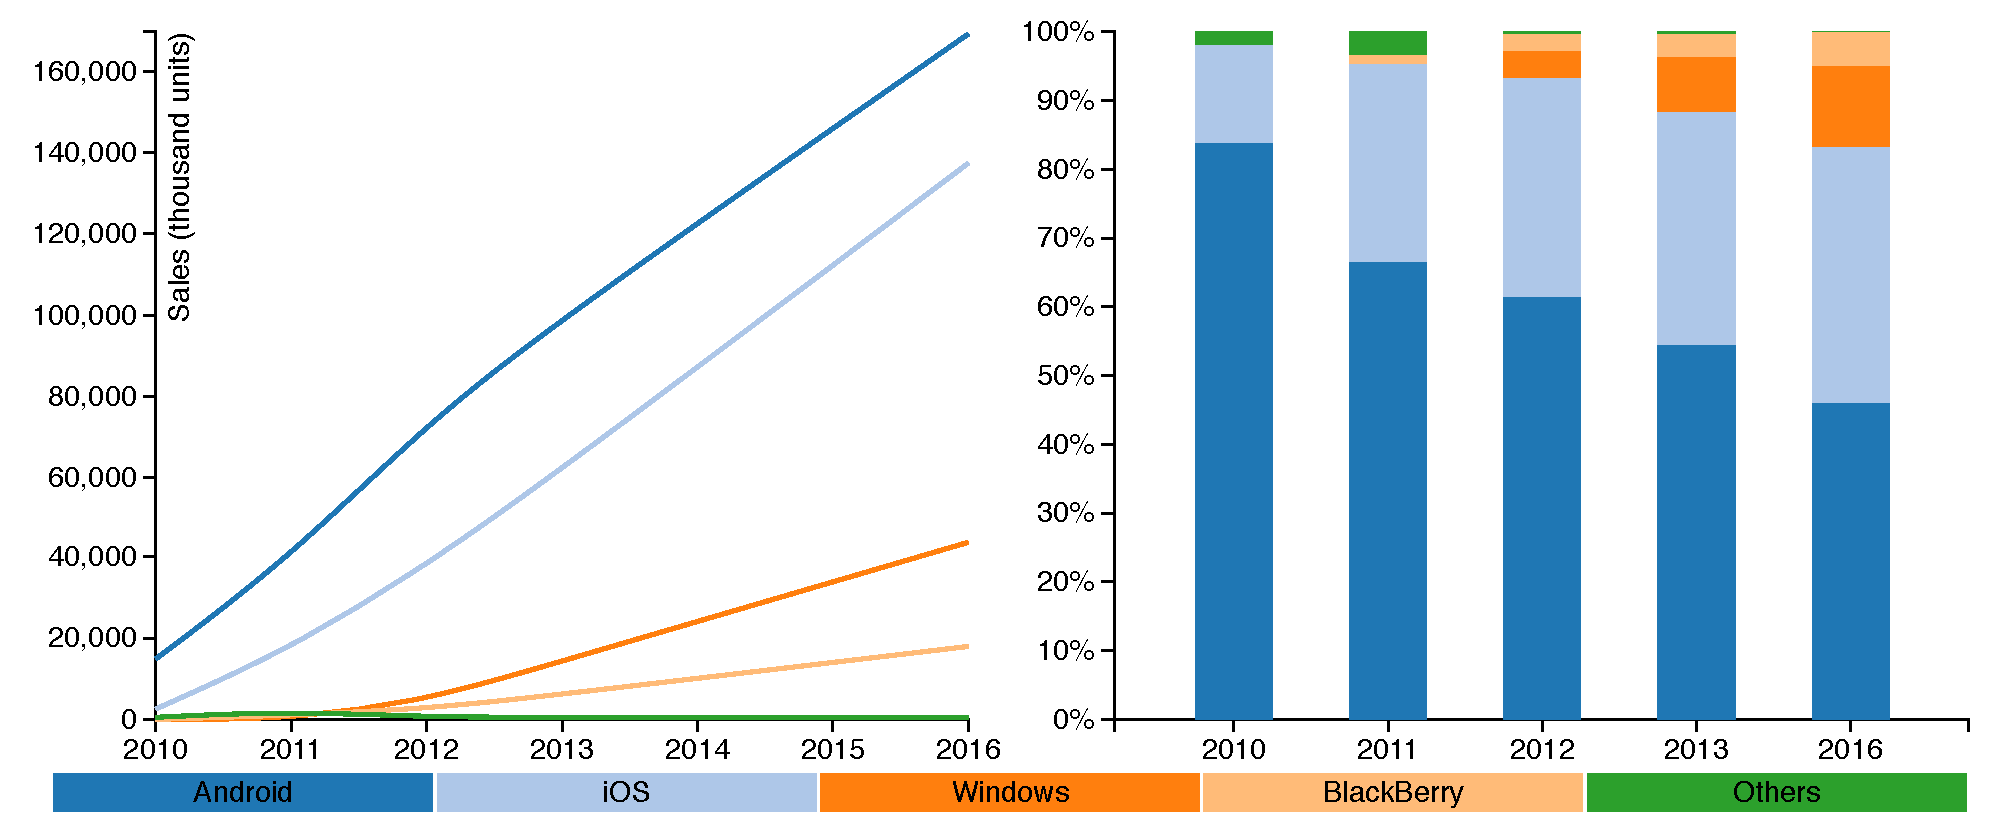
\includegraphics[width=\textwidth]{../resources/figs/tablet_sales.pdf}
    \caption{Prediction of worldwide tablet sales and market share.\newline Source: Gartner \citeGartnerTab}
    \label{fig:tablet}
\end{figure}

\section{The problem of fragmentation}

Fragmentation can be defined as the fact that all devices are different; there is no uniform device. This is called device fragmentation. In fact, all mobile devices can be divided into multiple, overlapping categories like operating system or platform (called platform fragmentation), operating system version or runtime (called runtime fragmentation), screen size and screen resolution (called screen fragmentation) and many more. Hence, fragmentation is a multi-dimensional problem. 

Fragmentation is generally beneficial for consumers, carriers and manufacturers. The more different devices there are, the more likely a consumer will find a device that fits his needs. For developers on the other hand, fragmentation is usually disadvantageous. It forces them to test their applications on multiple devices to guarantee the desired user experience. This is expensive and time-consuming. 

The nature of a platform strongly influences the fragmentation issues within said platform. For instance, Apple can manage fragmentation issues pretty well because iOS is a closed platform and the only devices running iOS, called iDevices, are designed by Apple itself. In fact, these devices show many similarities. Android on the other hand is an open system. Android is being developed privately at Google, but the source code of every release is publicly available under the Apache 2.0 License, which means that everybody is allowed to customize it. The ability for manufacturers to alter the operating system has largely contributed to the success of Android. 

Mobile device manufacturers are eager to modify the Android operating system to differentiate their product from their competitors. As such, they create their own Android flavour, i.e. a distribution of Android with a custom user interface (like HTC Sense, Samsung TouchWiz, etc.), custom software, additional market places, etc. However, reapplying these modifications for every new release of Android is cumbersome and costly which is why device manufacturers do not often provide updates for their devices. This has led to the notorious Android runtime fragmentation, which is depicted in \fref{fig:android_runtimes}. The adoption rate for new versions is low and is caused by the nature of Android. Developers have to support multiple versions, which is tedious. 

\begin{figure}[h]
    \centering
    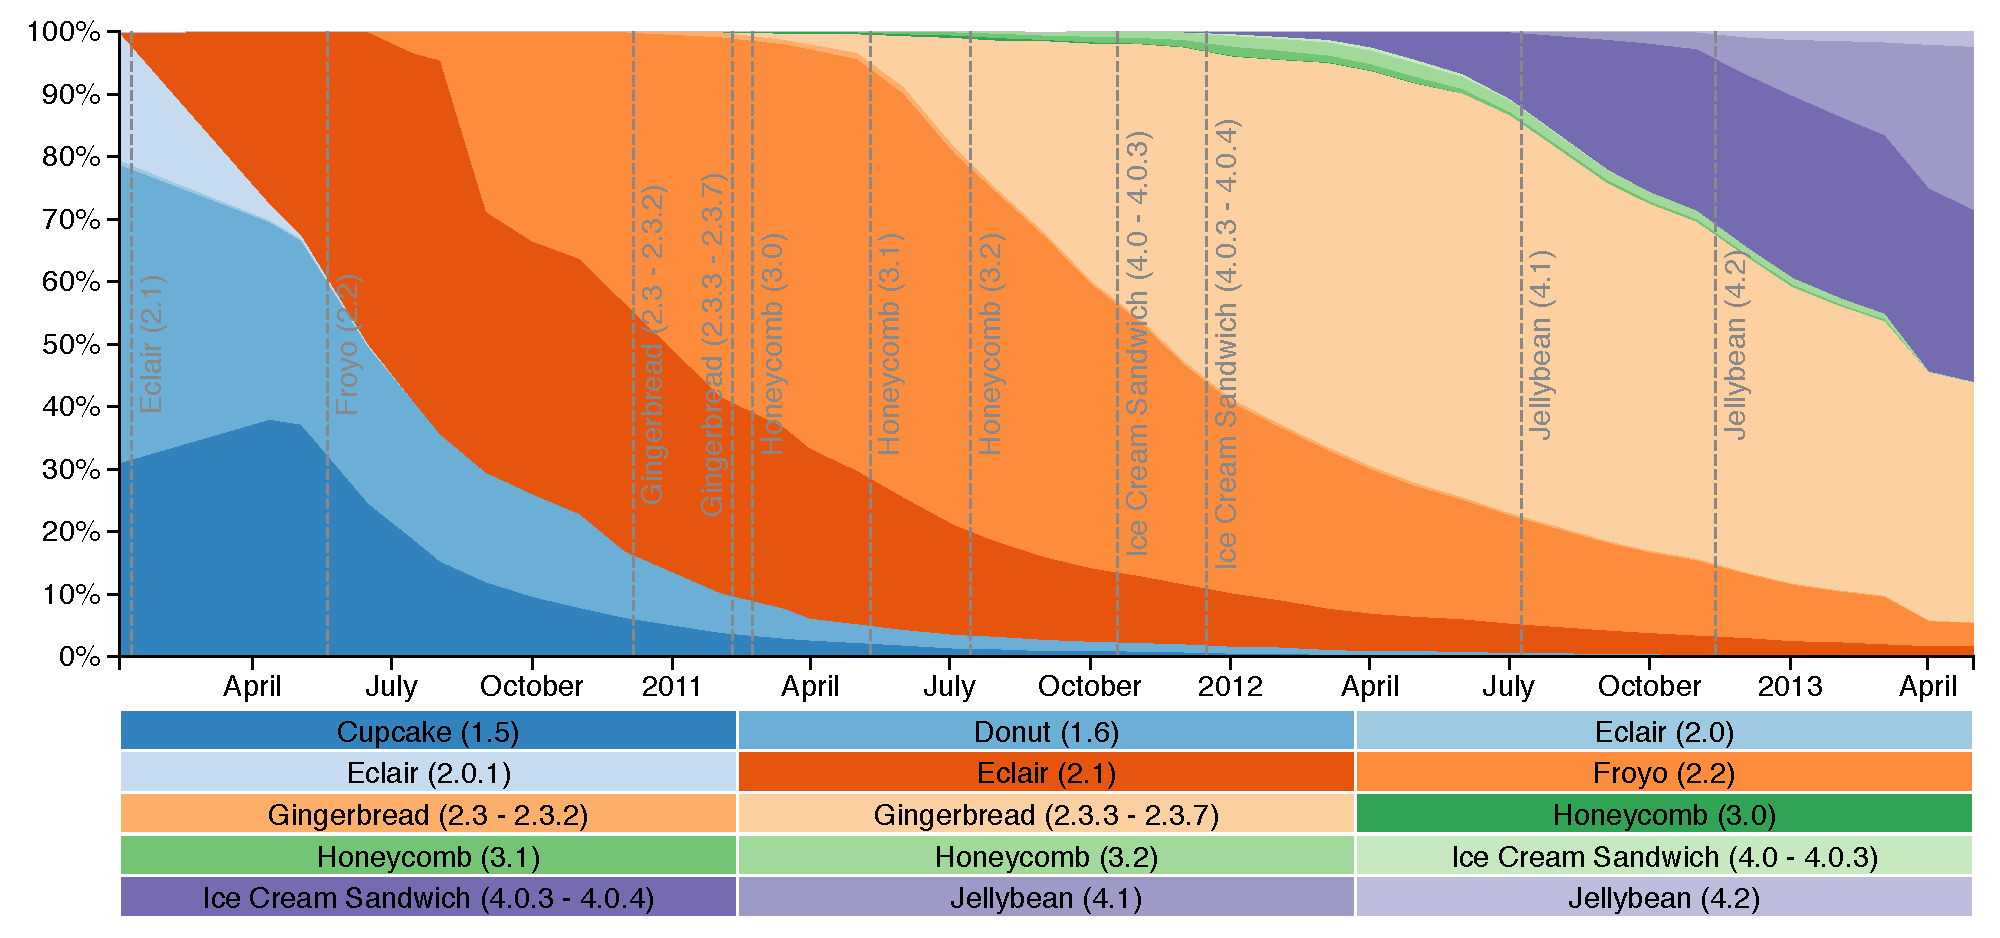
\includegraphics[width=\textwidth]{../resources/figs/android_runtimes.pdf}
    \caption{Historical Android runtime fragmentation. The data for this graph was aggregated from \cite{Android:Versions} using the Internet Archive (\url{http://archive.org}).}
    \label{fig:android_runtimes}
\end{figure}

Unlike Google, Apple does not publicize runtime statistics but developers \cite{Smith:2013} and online advertisers \cite{Chitika:2013} can confirm fast adoption rates for iOS. On iOS, developers can make use of new functionality much faster. However, as Apple starts to drop support for some of its devices that are still in use (like for instance the original iPad and the iPod third generation), it introduces runtime fragmentation. Because of this, iOS developers will have to support the latest two versions of iOS.

Android and iOS are used in both smartphones and tablets. There are only few different iDevices  but in contrast, there is an enormous number of Android devices. The Google Play Store\footnote{Google Play is the official marketplace for Android applications.} supports 2935 different device configurations, distributed across 63 manufacturers. All these devices come  with varying screen sizes and resolutions which implies that applications also have to deal with this. On Android, this is solved by a flexible layout system. On iOS, this is solved by centering the user interface in the middle of the screen. For instance, applications that are not optimized for the 4-inch display of the iPhone 5 (or iPod Touch, 5th generation) will have black bars on the top and the bottom. High-density displays\footnote{A high-density display has about twice the pixel density of a regular display.}, like the Retina display, do not really introduce a new screen resolution because every logical pixel is represented by four physical pixels and this conversion is mostly handled by the operating system.

There are still a lot more dimensions to the fragmentation problem like computing power, available sensors, available networking, etc. but these differences can be categorized under device fragmentation. In conclusion, fragmentation among Android devices is rather high compared to iDevices.

\section{Cross-platform tools to the rescue}

In the current economy, information is a company's most valuable asset and the rate at which information exchange takes place increases every day. Mobile Internet-enabled devices are a valuable resource for this purpose and, as a consequence, many companies want mobile applications for their businesses. However, in an ever-changing and unpredictable industry like the mobile industry, it is unwise to target a single platform. This could eventually lead to vendor lock-in, i.e. all operations (or a significant part thereof) are built on equipment or software of a single vendor which puts that vendor in a bargaining position. Companies will try to avoid these situations at all costs and they will do so by asking for cross-platform solutions. 

Making a solution work across platforms typically requires that the software has to be implemented multiple times: one time for each platform. This is costly and time-consuming. Cross-Platform Tools (CPTs) can help to solve this problem because they allow to support multiple platforms from a single codebase. Hence, they lower entry barriers (access to new platforms) and exit barriers (lock-in) \cite{VMCPT:2012}. 

Cross-Platform Tools try to solve three major problems \cite{VMCPT:2012}: 

\begin{enumerate}
    \item \textbf{Fragmentation} Fragmentation issues, as described above, are a struggle for every developer. They are forced to test their applications on a large number of devices in order to be able to guarantee the desired user experience. A CPT can help to identify platform quirks and provide workarounds. 
    \item \textbf{Access to new platforms} Targeting a new platform is generally hard. Developers have to learn yet another SDK and/or programming language in order to deliver applications for this platform. A CPT can make abstraction of platform differences which allows developers to reuse their current skills. This drastically reduces the effort that is needed to target a new platform. Bear in mind that a new platform does not necessarily have to be a smartphone or tablet operating system, it could also be the operating system of a television set, or a car console, etc.
    \item \textbf{Development inefficiency} Maintaining codebases for multiple platforms is a difficult and costly task. When a new feature is introduced, it has to be applied to all codebases. With the use of a CPT, all code is contained within a single codebase and no time is lost while synchronizing features and executing other maintenance tasks across codebases. This reduces cost while increasing productivity. 
\end{enumerate}

\section{Goals}

It is clear that there is a large demand for cross-platform solutions and that there are a lot of benefits associated with the use of cross-platform tools. Therefore, this thesis will try to identify a suitable cross-platform tool for mobile application development. This is a two-step process. First, a methodology will be defined for evaluating and selecting cross-platform tools. Second, this methodology will be used to evaluate two cross-platform tools (Apache Cordova and Motorola Rhodes) and the native SDK's in a business environment, provided by Capgemini\footnote{Capgemini is a multinational IT consulting company, \url{http://www.capgemini.com}.}. From this evaluation, the best-suited alternative will be selected. 
\chapter{Literature Study}
\label{chap:literature}

\npar The mobile industry is without a doubt one of the most vibrant industries at the moment. Not only because mobile device sales are growing rapidly but also because of the highly competitive nature of this market. This has led to fragmentation. 

\npar This chapter will sketch the landscape of mobile devices, explain the problem of fragmentation and a number of suggested solutions to cope with this problem.

\section{The mobile device landscape}

\npar In the last couple of years, smartphone sales have gone up quickly. Smartphones are becoming ubiquitous and in some regions, like the United States, smartphone penetration has already reached more than 50\% \cite{Nielsen:2012}. According to quarterly studies by Gartner, smartphone penetration remained stable before the iPhone 3G and Android came along (see \fref{fig:smartphone_sales}).

\begin{figure}[h!]
    \begin{center}
        \includegraphics[width=\textwidth]{figs/smartphone_sales.pdf}
        	\caption{
        	    	Growth of worldwide smartphone sales and smartphone penetration. Source: Gartner \citep{Gartner:08Q2,Gartner:08Q3,Gartner:08Q4,Gartner:10Q1,Gartner:10Q2,Gartner:10Q3,Gartner:10Q4,Gartner:11Q1,Gartner:11Q2,Gartner:11Q3,Gartner:11Q4,Gartner:12Q1,Gartner:12Q2}
        	}
        	\label{fig:smartphone_sales}
    \end{center}
\end{figure}

\begin{figure}[h!]
    \begin{center}
        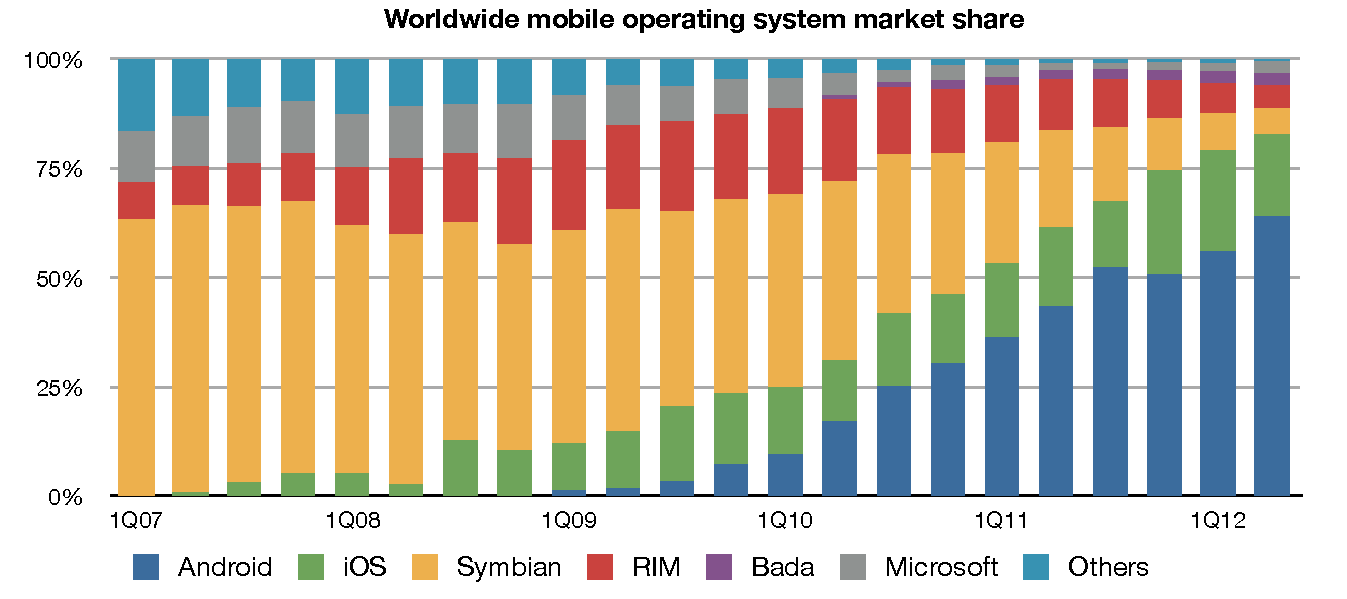
\includegraphics[width=\textwidth]{figs/smartphone_os.pdf}
        \caption{
            Growth of worldwide smartphone operating system market share. Source: Gartner \citep{Gartner:08Q2,Gartner:08Q3,Gartner:08Q4,Gartner:10Q1,Gartner:10Q2,Gartner:10Q3,Gartner:10Q4,Gartner:11Q1,Gartner:11Q2,Gartner:11Q3,Gartner:11Q4,Gartner:12Q1,Gartner:12Q2}
        	}
        \label{fig:smartphone_os}
    \end{center}
\end{figure}

\npar But more importantly, one can conclude that there is not one major platform. Projections by the IDC show that in 2016, there will be at least three major platforms covering 90\% of the worldwide smartphone market \citep{IDC:phone}. 

\npar A similar scenario is playing in the tablet industry. According to other studies by both Gartner \citep{Gartner:11tab,Gartner:12tab} and IDC \citep{IDC:tablet}, tablets will continue to gain popularity and sales will be mainly driven by iPads and Android tablets (see \fref{fig:tablet}).

\begin{figure}[h!]
    \begin{center}
        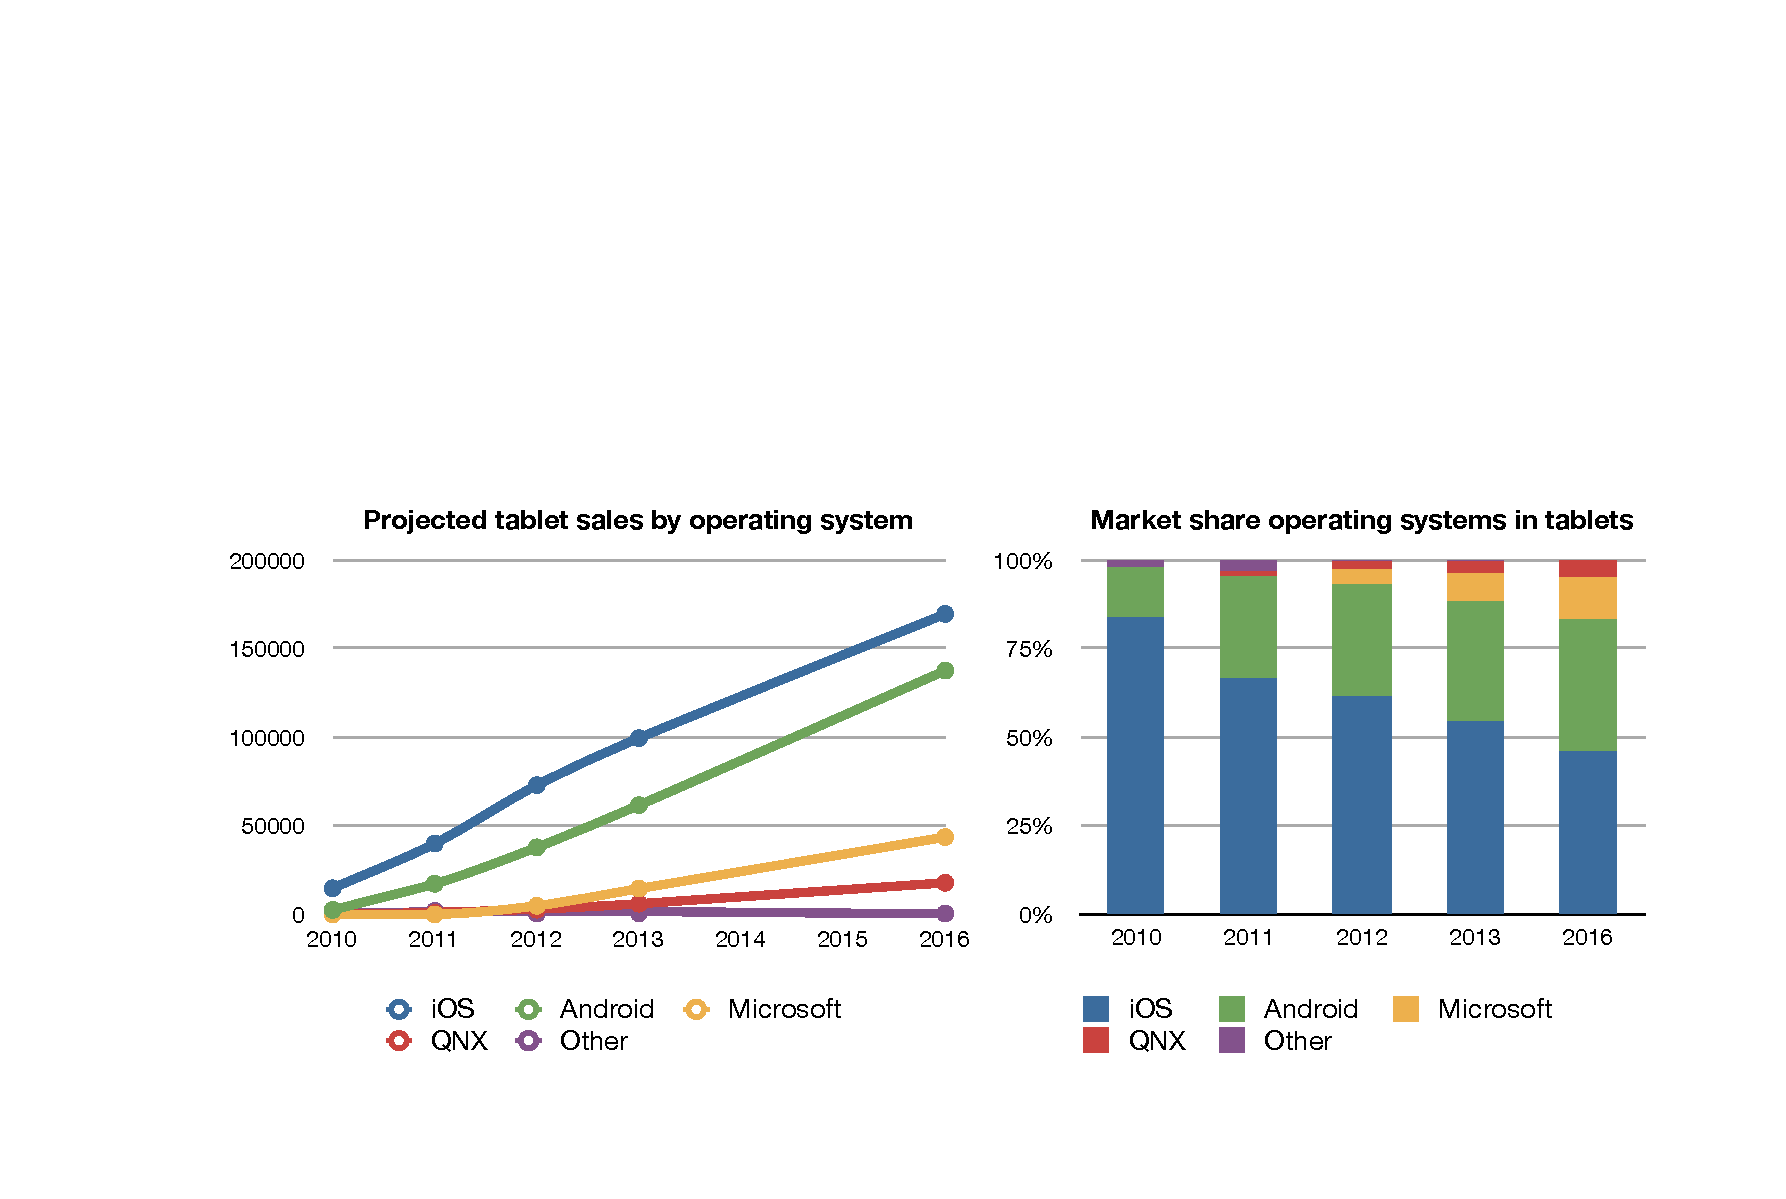
\includegraphics[width=\textwidth]{figs/tablet.pdf}
        \caption{
            Growth of worldwide smartphone sales and smartphone penetration. Source: Gartner \citep{Gartner:11tab,Gartner:12tab}
        }
        \label{fig:tablet}
    \end{center}
\end{figure}

\npar Even though both companies do not agree on which platform will be the biggest by 2016, they both predict there will be at least three major platforms; iOS, Android and Windows. 

% TODO: summary?

\section{The problem of fragmentation}

\npar The competition among mobile device manufacturers has led to fragmentation on many levels. For consumers, fragmentation is usually a good thing. The more different devices there are, the easier it is for a consumer to pick one that fits his needs. For developers on the other hand, fragmentation is usually considered bad. Developers have to develop and test their applications on multiple devices to be able to guarantee the desired experience. This is expensive and time consuming.

\npar From \fref{fig:smartphone_os} and \fref{fig:tablet} it is already clear that the market is divided by operating system or platform but even within these platforms, fragmentation is multi-dimensional \citep{Kindel}.

\npar In general, there are fewer fragmentation problems with Apple's iOS because it is a closed platform. Android, however, is an open source platform and vendors are allowed to tailor it for their devices. As a result, there are hundreds of Android based devices but also hundreds of Android flavours.

\npar Maintenance of such Android flavours is expensive and for this reason, manufacturers do not often provide updates for their devices. This has led to noticeable runtime fragmentation among Android based devices (see \fref{fig:runtime_fragmentation}). Compared to iOS, this is a serious issue.

\begin{figure}[h!]
    \begin{center}
        \label{fig:runtime_fragmentation}
        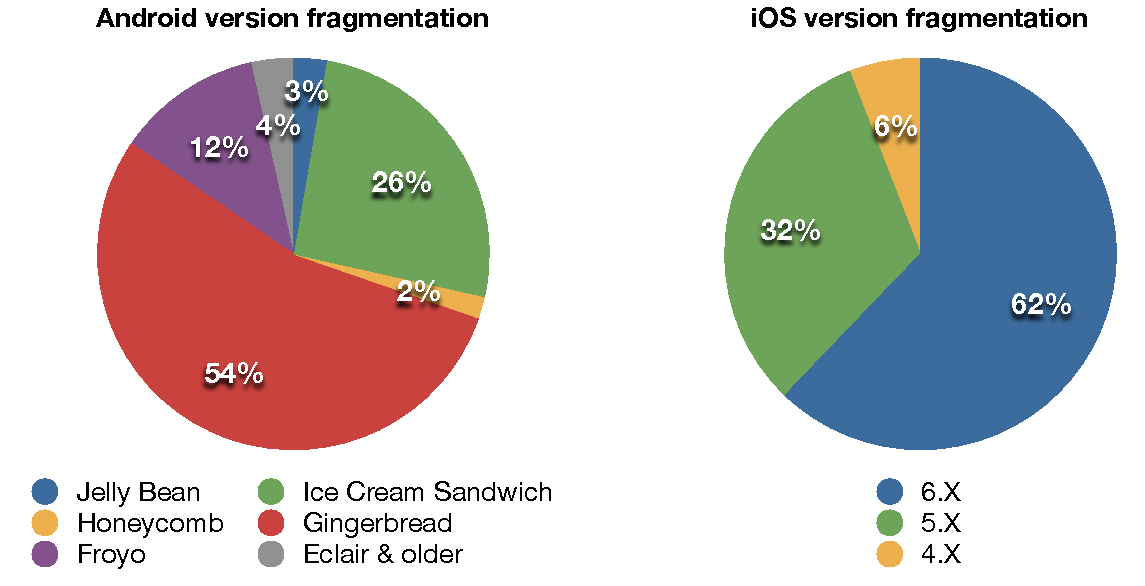
\includegraphics[width=0.8\textwidth]{figs/os_distribution.pdf}
        \caption{
            Runtime fragmentation for Android (data collected by Google during a 14-day period ending on November 1, 2012) \citep{android_distribution} and iOS (based on the statistics of developer David Smith) \citep{ios_distribution}.
        }
    \end{center}
\end{figure}

\npar Fragmentation on the device axis is unavoidable but, again, fragmentation among Android based devices is worse than among iDevices. The most relevant items on this axis are the different hardware specifications and screen resolution.

\npar 

\section{Strategies for cross platform development}

\npar There are already a number of paradigms for cross platform mobile application development \citep{Friese}. This section presents an overview of the available strategies by comparing different aspects: performance, look and feel, platform access, programming languages, development cost and distribution.

% TODO: discuss development cost

\subsection{Native App}

\npar A native app is an application that is specifically designed to run on a particular platform. It is the default approach to develop applications for mobile devices. \fref{fig:native} shows an illustration of the overall architecture of such an app. 

\begin{figure}[h!]
    \begin{center}
        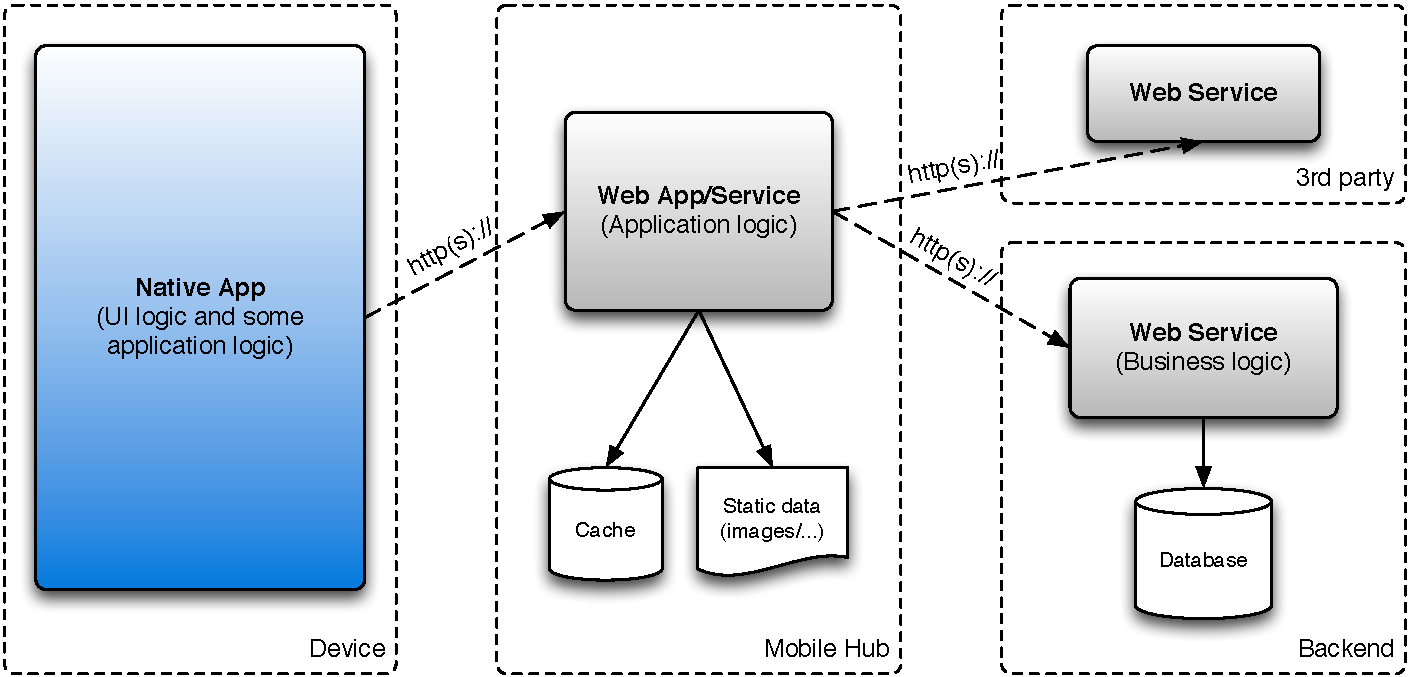
\includegraphics[width=\textwidth]{figs/native.pdf}
        \caption{
            Overall architecture of a native app. 
        }
        \label{fig:native}
    \end{center}
\end{figure}

\npar Native apps are developed with the supplied SDK. Developers will need to get acquainted with the programming language used by said SDK but in return they will get full access to the platform and its features. As a result, the best performance can be obtained with this kind of app.

\npar For the user interface, developers can use lots of interface elements such that they can present a familiar look and feel to the end user. 

\npar Native apps can be easily distributed through an online marketplace like for instance the App Store or Google Play. 

\npar Because native apps are designed to run on one platform only, this development strategy is not very well suited for cross platform development. If an application should run on multiple platforms, it has to be developed for each platform separately. This is costly.

% TODO: talk about mobile hub

\subsection{Web App}

\npar Web apps are websites that are optimized for mobile browsers. Since every platform comes with a browser, this is the easiest way to get an application running on all platforms. An overview of the overall architecture for this kind of app is given in \fref{fig:web}.

\begin{figure}[h!]
    \begin{center}
        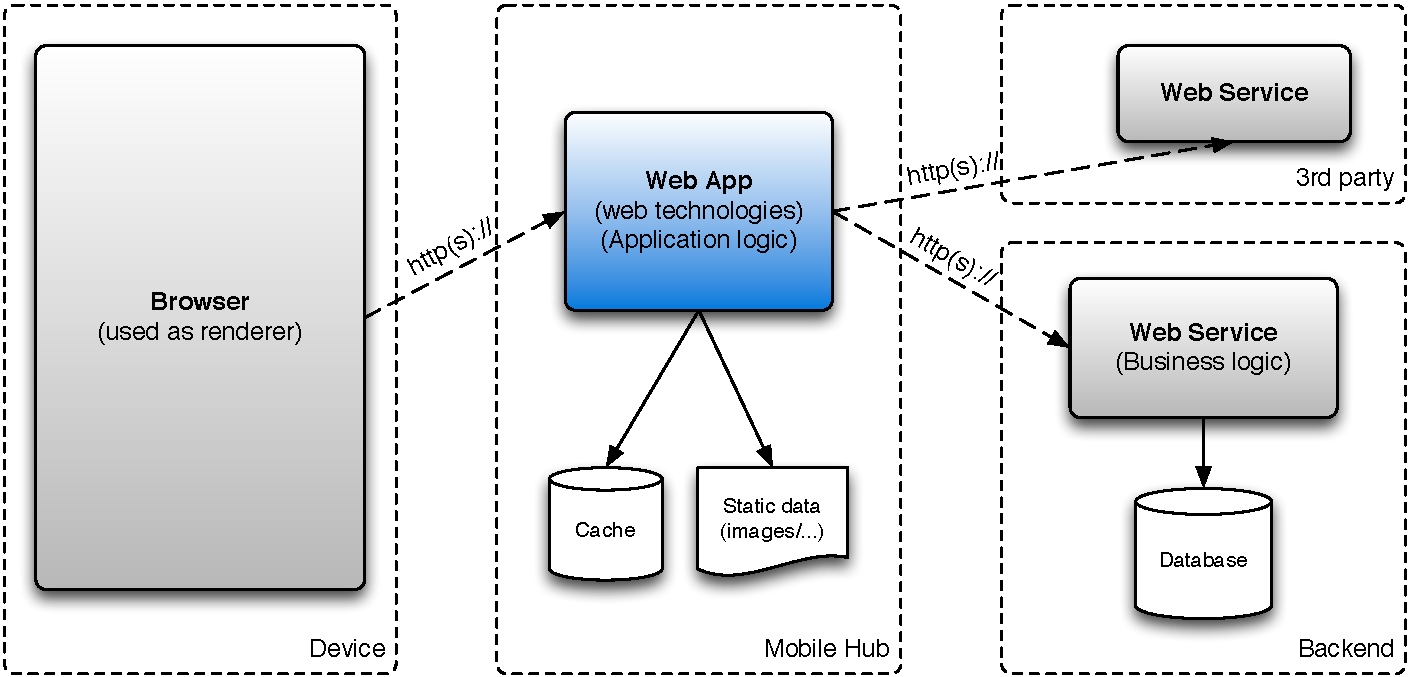
\includegraphics[width=\textwidth]{figs/web.pdf}
        \caption{
            Overall architecture of a web app.
        }
        \label{fig:web}
    \end{center}
\end{figure}

\npar Web apps are not nearly as powerful as native apps. First of all, the application is not stored on the device. Web apps require an active internet connection which cannot always be guaranteed. Second, they are built with web technologies like HTML, CSS and JavaScript, which have to be interpreted by the browser at runtime. Third, web apps cannot access the system which means they cannot make use of the many unique features of a mobile device. 

\npar With HTML5, web apps can get more powerful. They will be able to access device features, like the camera and other sensors \citep{MobileHTML5}. They will not even require an active internet connection because they can be cached on the device. However, HTML5 is still a draft and a lot of mobile browsers lack proper HTML5 support.

\npar From a user interface perspective, web apps can be a problem as well. % TODO: complete paragraph

\npar Web apps are distributed easily: the only requirement is a valid URL. Web apps cannot be installed on the device though, but there are workarounds using Web Clips on iOS \citep{Safari:webclips} and bookmarks on Android. 

\subsection{Hybrid App}

\npar Hybrid applications are the logical next step, combining native apps and web apps. The actual application is a web site, embedded in a web view, part of a native wrapper. The embedded website can access (parts of) the system through a bridge. An overview of the overall architecture is shown in \fref{fig:hybrid}. 

\begin{figure}[h!]
    \begin{center}
        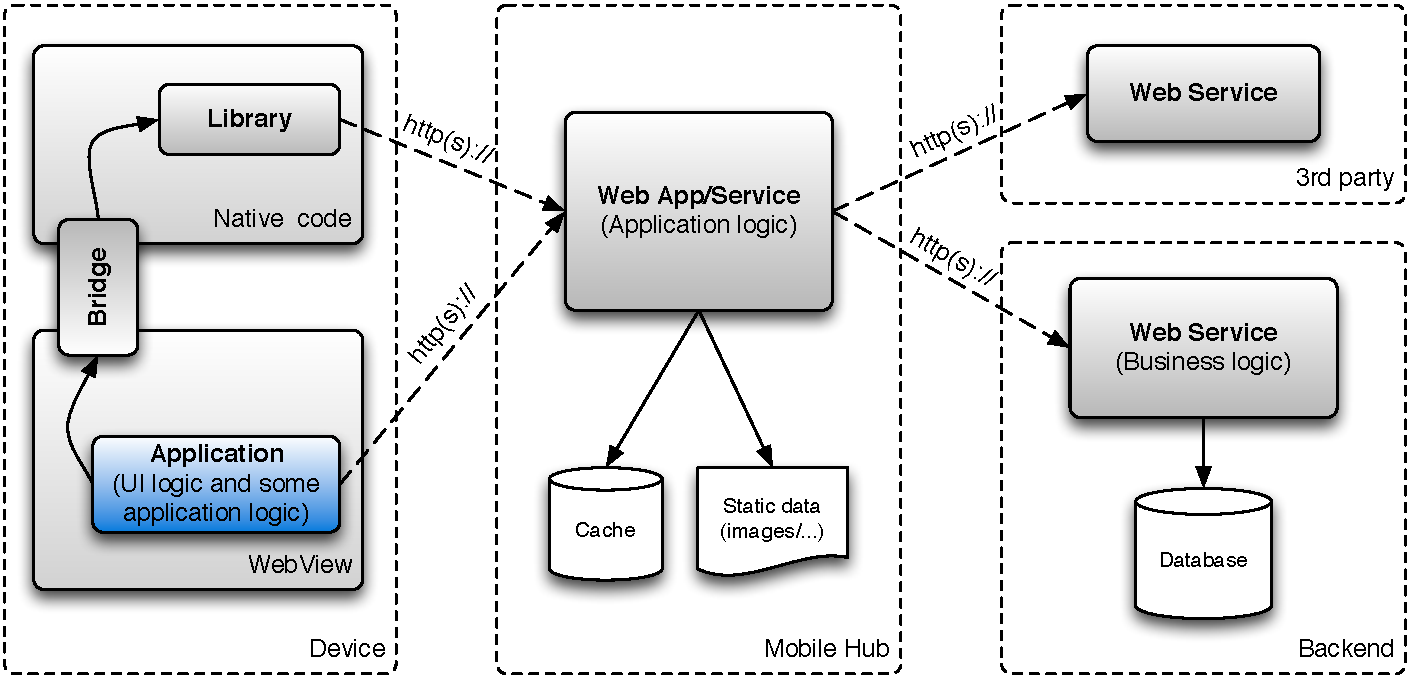
\includegraphics[width=\textwidth]{figs/hybrid.pdf}
        \caption{
            Overall architecture of a hybrid app.
        }
        \label{fig:hybrid}
    \end{center}
\end{figure}

\npar Hybrid apps are part native app, part web app. Performance will be similar to web apps but some parts can be optimized by using native code. The websites inside the hybrid app are also much more powerful because they can access many device features that aren't available in HTML(5) through the bridge.

\npar When it comes to the user interface, hybrid apps suffer from the same problem as web apps. 

\npar Because hybrid apps are wrapped in a native container, they can be distributed just like native applications, through online marketplaces. 

\subsection{Interpreted App}

\npar In an interpreted app, instructions in some language are translated to native instructions at runtime. \fref{fig:interpreted} shows the overall architecture of an interpreted app.

\begin{figure}[h!]
    \begin{center}
        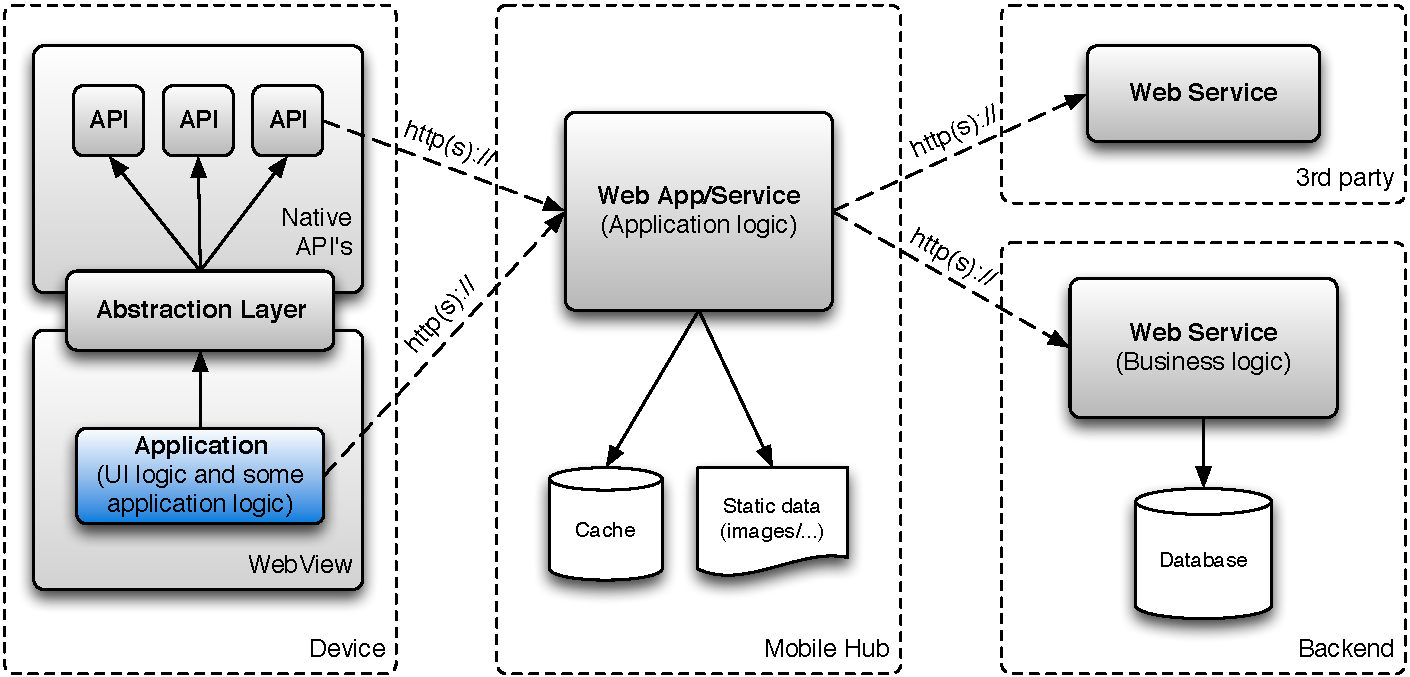
\includegraphics[width=\textwidth]{figs/interpreted.pdf}
        \caption{
            Overall architecture of an interpreted app.
        }
        \label{fig:interpreted}
    \end{center}
\end{figure}

\npar Performance of interpreted apps depends on the interpreter and interpreted language but is better than web apps on average, though not as good as native apps. 

\npar In an interpreted app, the user interface description is interpreted and rendered on the device using native interface elements. An interpreted app will have a familiar look and feel.

\npar From the outside, interpreted apps -- just like hybrid apps -- look like native apps and can be distributed through online marketplaces.

\subsection{Cross Compiling}

\npar Instead of translating instructions at runtime, one could translate instructions at compile time. The process is called cross compiling and the result is a truly native app. The overall architecture is sketched in \fref{fig:crosscompiled}. 

\begin{figure}[h!]
    \begin{center}
        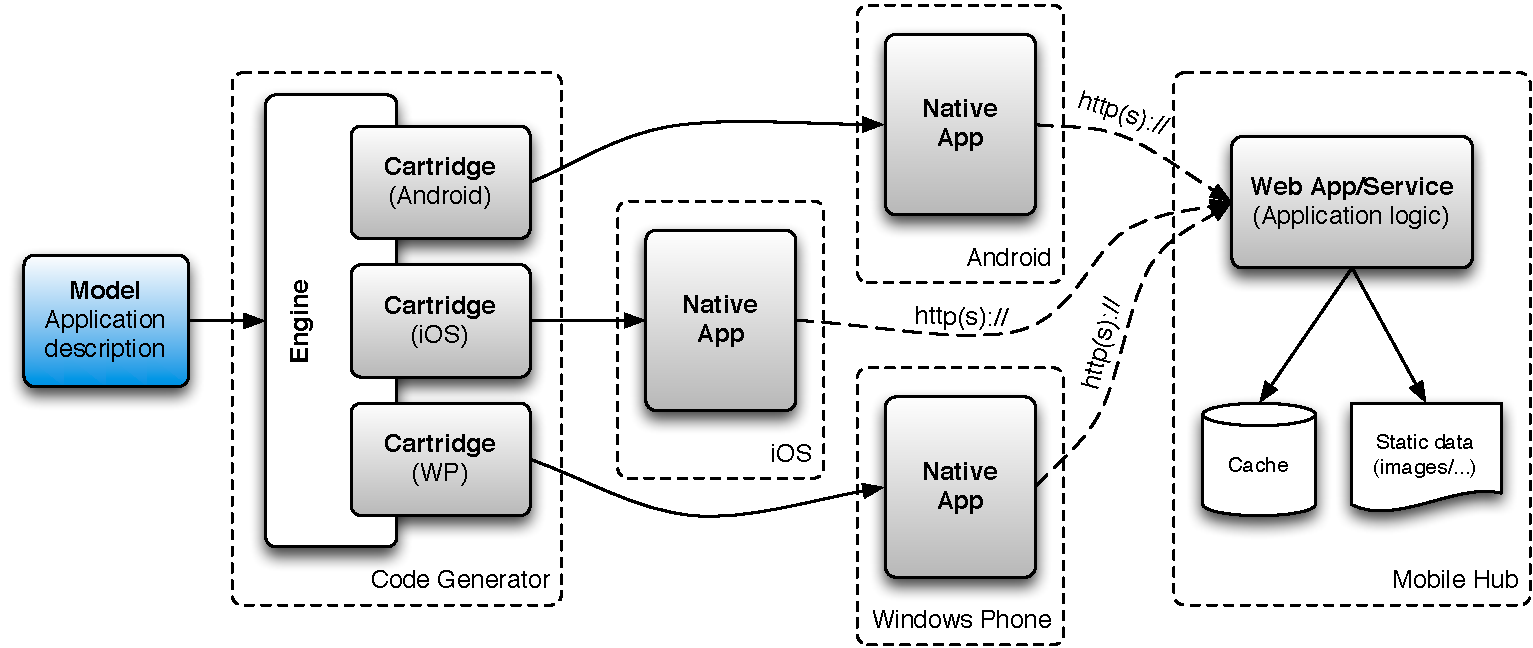
\includegraphics[width=\textwidth]{figs/crosscompiled.pdf}
        \caption{
            Overall architecture for cross compiled apps. 
        }
        \label{fig:crosscompiled}
    \end{center}
\end{figure}

\npar 

\subsection{Summary}

\tref{tab:architectures} summarizes the results of the discussed strategies. It is important to note that there is no universal strategy that fits all use cases. A strategy must be chosen carefully, taking into account the client's wishes.

\begin{table}[h!]
    \begin{center}
        \begin{tabular}{l|c|c|c|c|c}
                             & Native      & Web                   & Hybrid      & Interpreted & Cross Compiled\\
            \hline
            Performance      & high        & low                   & rather low  & average     & high          \\
            Platform Access  & \checkmark  & $\times$ / \checkmark & \checkmark  & \checkmark  & \checkmark    \\
            Look \& Feel     & native      & non-native            & non-native  & native      & native        \\
            Distribution     & marketplace & URL                   & marketplace & marketplace & marketplace   \\
            Development cost & high        & rather low            & average     & average     & average       \\
        \end{tabular}
		\caption{
			Summary of cross platform mobile application development strategies.
		}
		\label{tab:architectures}
    \end{center}
\end{table}

\npar

\section{Conclusion}
%\include{chap-2}
% ... and so on until
%\include{chap-n}
%\chapter{Conclusion}
\label{chap:conclusion}

This final chapter presents a summary of the work, together with a critical reflection and an overview of potential future improvements. 

\section{Goals}
\label{sec:goals}

This thesis had two major goals. The first goal was to design a methodology for evaluating and selecting a cross-platform tool for mobile application development. The second goal was to use this methodology to evaluate real cross-platform tools and select the most suited candidate. The methodology that was used is inspired by the generic software package selection, presented by \citet{Jadhav:2011}, and comprises of six highly customizable stages. Each of these stages has been concretized in Chapter \ref{chap:methodology}. 

During the first stage, the selection criteria were gathered. These are the most essential requirements that a cross-platform tools has to meet. The selection criteria were defined by Capgemini and require cross-platform tools to produce native applications for both Android and iOS and for both smartphones and tablets. 

During the second stage, a list of potential candidates was composed from Internet searches and literature. An extensive list of cross-platform tools was found in ``Cross-platform developer tools 2012'', a report by VisionMobile on this subject \cite{VMCPT:2012}. Subsequent Internet searches did not reveal new tools.

During the third stage, this list of potential candidates was filtered using the selection criteria from the first stage and from the resulting list, two cross-platform tools were selected for evaluation. These tools are Apache Cordova and Motorola Rhodes (see Chapter \ref{chap:tools}). The native development kits for both Android and iOS were also included as a baseline for the evaluation. 

During the fourth stage, the evaluation criteria were defined. Three people at Capgemini were interviewed: a developer, a mobile architect and a sales person. From these interviews and literature, eleven evaluation criteria were identified: platform support, toolset reuse, code reuse, access to hardware, integration with platform-specific services, native look \& feel, user interface capabilities, performance, skill reuse, tooling and testing. These criteria are organized in a hierarchy because humans can only process 7 plus or minus 2 pieces of information at the same time.

During the fifth stage, the alternatives were evaluated using these evaluation criteria. For this evaluation, the Analytic Hierarchy Process (AHP) \cite{Saaty:1980} was used. This method assigns weights to both criteria and alternatives based on judgements that originate from pairwise comparisons. In order to formulate a reliable judgement, a proof-of-concept application was implemented with the studied tools. The evaluation is carried out from two perspectives: one from the perspective of a developer, one of a perspective of a mobile architect. Both could have different opinions about cross-platform tool qualities, which could result in a different ranking.

During the sixth and last stage, the candidates that is are most suited were carefully selected. This required a cost-benefit analysis to ascertain that the selected alternative was also cost-effective. For this cost-benefit analysis, development time was used as a cost driver and the scores for the alternatives, obtained from the evaluation, were used as benefits. From this analysis, it was concluded that Apache Cordova is currently equally cost-effective as the native development kits when only targeting Android and iOS. However, if in the future a third platform has to be supported, Cordova will be more cost-effective because the application can be completely reused on the next platform.

\section{Reflection and future work}
\label{sec:reflection}

The methodology presented in this thesis ends with the selection of a cross-platform tool. However, the usefulness of this tool is never validated. Hence, a seventh, validation stage seems desirable. However, it is not possible to include this step in the timeframe of this thesis because such validation requires that the tool is used in a production environment for quite some time. The prolonged use of a particular tool in a large-scale environment will definitely reveal more benefits and/or issues than a simple proof-of-concept application can in a small-scale and controlled environment. Ergo, this seventh step is of utmost importance after the selection of a cross-platform tool.

Also, the mobile industry is rapidly evolving, which inherently makes cross-platform tools moving targets. The outcome of this study will probably be different in one year from the moment of writing. This makes continuous evaluation of the available tools a necessity and introduces a feedback loop in the evaluation process. New technologies often provide less functionality in the early stages of its life cycle but they can quickly overcome the functionality of the current technologies. New tools can be deemed ineffective at a certain time, but may become more effective than the current tools in the future. Frequent reevaluation is a must.

From the cost-benefit analysis in this study it is concluded that Apache Cordova and the native development kits are currently equally cost-effective. If a company decides to use Cordova for a number of its applications, a new problem rises because Cordova only wraps (mobile) web applications. There is a large number of tools available for (mobile) web development. Working with each of these technologies will create a different experience, both for developers and end-users, which motivates the need for another comparative study, a study that compares tools for (mobile) web development. 

During the evaluation phase, the criteria are weighted using the judgements of only two individuals. The evaluation is based on the judgement of the evaluator. Hence, the result does not represent the animo among developers and architects. The result rather represents the combined judgement of three individuals. In future work, it might be wise to increase the sample size of the questioned people and evaluators in order to obtain a statistically valid result. However, having multiple individuals evaluate the alternatives was simply not an option and only two employees were available for questioning. 

For the evaluation, the Analytic Hierarchy Process is used. One of the strengths of this method is that it is based on pairwise comparison but this could also become a weakness when a large number alternatives needs to be evaluated. This problem can be solved either by using another evaluation technique or by making modifications to the AHP to deal with these numbers, as is suggested in literature.






% If you have appendices:
% optional appendix separator page
\appendixpage*

\appendix

%\chapter{The First Appendix}
\label{app:A}


% ... and so on until
%\include{app-n}

\backmatter
% The bibliography comes after the appendices.
% You can replace the standard "abbrv" bibliography style by another one.
\bibliographystyle{plainnat}
\bibliography{references}

\end{document}